%%%%%%%%%%%%%%%%%%%%%%%%%%%%%%%%%%%%%%%%%
% University/School Laboratory Report
% LaTeX Template
% Version 3.1 (25/3/14)
%
% This template has been downloaded from:
% http://www.LaTeXTemplates.com
%
% Original author:
% Linux and Unix Users Group at Virginia Tech Wiki 
% (https://vtluug.org/wiki/Example_LaTeX_chem_lab_report)
%
% License:
% CC BY-NC-SA 3.0 (http://creativecommons.org/licenses/by-nc-sa/3.0/)
%
%%%%%%%%%%%%%%%%%%%%%%%%%%%%%%%%%%%%%%%%%

%----------------------------------------------------------------------------------------
%	PACKAGES AND DOCUMENT CONFIGURATIONS
%----------------------------------------------------------------------------------------

\documentclass{article}

\usepackage[version=3]{mhchem} % Package for chemical equation typesetting
\usepackage{siunitx} % Provides the \SI{}{} and \si{} command for typesetting SI units
\usepackage{graphicx} % Required for the inclusion of images
\usepackage{natbib} % Required to change bibliography style to APA
\usepackage{amsmath} % Required for some math elements 
\usepackage[a4paper,bindingoffset=0.2in,%
            left=1in,right=1in,top=1in,bottom=1in,%
            footskip=.25in]{geometry}
\usepackage[hidelinks]{hyperref}
\setlength\parindent{0pt} % Removes all indentation from paragraphs

\renewcommand{\labelenumi}{\alph{enumi}.} % Make numbering in the enumerate environment by letter rather than number (e.g. section 6)

%\usepackage{times} % Uncomment to use the Times New Roman font

%----------------------------------------------------------------------------------------
%	DOCUMENT INFORMATION
%----------------------------------------------------------------------------------------

\title{Report of Sketches Experiment} % Title

\author{Zhendong \textsc{Liu} A0159369L} % Author name

\date{\today} % Date for the report

\begin{document}

\maketitle % Insert the title, author and date

\section{Introduction}
This report makes conclusion of the experimenting result of two different sketch algorithms towards the streaming problem on problem set 1.1, where we use a set of 1-sparse samplers to count the appearance times of an item in a stream.
\newline
\newline
In this experiment, we tested the two algorithms on both uniform distribution input stream and exponential distribution input stream. By design a $correctRate$ standard on measuring the accuracy of algorithms and specifying many possible value of the parameters $M, N, A, B$, we see the overall performance of algorithms under different conditions.
\newline
\newline
We find that whether algorithm2 is better than algorithm1 on accuracy is depend on the value of $N$ and $B$, but have no relevance with the distribution of the items in stream or the different items in stream. For detailed conclusions and discussion please refer to section 5.
\newline
\newline
The source code wrote by myself is on Github:\\\url{https://github.com/lzddzh/cs5234/blob/master/pset4/countItemFrequncy.py}
% If you have more than one objective, uncomment the below:
%\begin{description}
%\item[First Objective] \hfill \\
%Objective 1 text
%\item[Second Objective] \hfill \\
%Objective 2 text
%\end{description}


 
%----------------------------------------------------------------------------------------
%	SECTION 2
%----------------------------------------------------------------------------------------

\section{Implementation}
We choose Python as the programming language for this project   since it is easy to write and we concern about the algorithms accuracy but not their speed (In general, Python program is not fast).
In the code, a $CounterSampler$ class has been implemented, with member variables stores the value of $A, B, P$(the prime number in hash functions), etc., and with several member functions such as $push(num), getResult(num), hash(num, a, b, P), etc$. We will not include the whole class here but only some key data structures will be introduced below.

\subsection{Counters}
It is easy to think about using a 2D array with unsigned int data type to implement the counters, since the counters count only positive values and the number of rows or columns of the counters won't change. Here what we use is a A * B sized numpy matrix with 0 initialled:
\begin{itemize}
\item $counters = numpy.zeros((A, B), dtype = 'uint64')$
\end{itemize}
Then access the i$^{th}$ row and j$^{th}$ column counter $C(i,j)$ by using $counters[i][j]$

\subsection{Hash functions}
Its fool's effort to directly store a big number of hash functions in a class. Instead we implement the hash functions by using a single member function and a member variable of our class:

\begin{itemize}
\item $hash(num, a, b)$
A member function that takes $num$ as its input and  returns $(ka * num + kb) \% Prime$. This hash function can be set with different paramaters $ka$ and $kb$. And the $Prime$ we choose is $Prime = min\{P|P>100*B,\ P\ is\ prime\}$, where $B$ is the number of columns of counters.
\item $parametersList = ((a_{1},b_{1}),(a_{2},b_{2}), ...)$
An array of tuples for storing the A hash functions parameters. In this array, we have A pairs of tuple (a,b), whose value are $1 \leq a, b \leq Prime$
\end{itemize}
 
To use the different hash functions, we just specify different pairs of (a,b) for the member function hash(num, a, b), $h_{i}(num) = hash(num, a_{i}, b_{i})$, so by storing A pairs of (a,b) in the member variable of $CounterSampler$ class, we can use any of the hash functions as we need.


\subsection{Two Algorithms}
Since the two algorithms are only different in their way of getting result from counters, we just use two different member functions $getResult1(num)$ and $getResult2(num)$ in the class $CounterSampler$ to get result from Algorithm1 and Algorithm2.

\begin{itemize}
\item $CounterSampler.getResult1(num)$ returns the minimum value among $C(i,h_i(num)$ for all $0\leq i\leq A-1$
\item $CounterSampler.getResult2(num)$ returns the median value of $Estimate(x,i)=C(i,h_i(num) - neighbor(C(i,h_i(num)))$ for all $0\leq i\leq A-1$
\end{itemize}


%----------------------------------------------------------------------------------------
%	SECTION 3
%----------------------------------------------------------------------------------------

\section{Test Design}

\subsection{Random Numbers for Test Data}
\begin{itemize}
\item $Uniformly Distribution$: We use the build-in Python function $random.randint(a,b)$ which generate a uniformly random number $r$ that $a \leq r \leq b$, and we just repeat this functions N times so we have N random numbers.
\item $Exponential Distribution$: We use the build-in Python function $numpy.random.exponential(\beta, size)$ to generate a list of random numbers that follows the exponential distribution $f(x)=\frac{1}{\beta}exp^{-\frac{x}{\beta}}$. Here we choose $size = N, \beta = \frac{M}{11}+1$, which let the output of random numbers are very likely to with in the range $0 \leq x \leq M$(if we are very not lucky and x exceeds M, we just re-generate it again). And since we need integers but not float numbers, so we going to just use the integers part of the generated numbers.
\end{itemize}

\subsection{Correct Rate}
If we want to compare the accuracy of two algorithms, we must have a standard. Here we use a $correctRate$ to represent the accuracy of the results output by one particular algorithm.

We define a the correct Rate on a given algorithm $K\in\{1,2\}$ and the set of numbers appeared in the input stream $Z = \{x_1, x_2, ..., x_n\}$ by 
\begin{equation}
	correctRate(K, Z) = \dfrac{\sum_{x\in Z} g(K, x)}{|Z|}
\end{equation}

\begin{equation}
    g(K,x)=\left\{
                \begin{array}{ll}
                  1\ (CounterSampler.getResultK(x) = n(x))\\
                  0\ (CounterSampler.getResultK(x) \neq n(x)) 
                \end{array}
              \right.
\end{equation}
where $n(x)$ is the times of $x$ appears in the stream, and $CounterSampler.getResultK(x)$ is the one in Section 2.3.

\subsection{Parameter Choosing}
There are four parameters in our algorithms that could influence the correct rate: $M, N, A, B$, separately represents the maximum number in the stream, the length of the stream, the rows of counters and the columns of counters. We want to see how algorithms works on different values of this parameters, so we choose each of these variables a range of values to test the two algorithms.

\begin{itemize}
\item $M$: we will test $M \in \{10, 100, 1000, 10000\}$
\item $N$: we will test $N \in \{10, 100, 1000, 10000\}$
\item $A$: we will test $A \in \{3, 4, 7, 10, 100\}$
\item $B$: we will test $B \in \{10, 20, 40, 80, 160, 500, \}$
\end{itemize} 

For each kind of test data set. First we are going to fix A and B then test the combinations of values in $M$ and values in $N$, see the correct rate of Algorithm1 and Algortihm2. Next, we will fix M and N then test the combinations of values in $A$ and values in $B$, see the correct rate of Algorithm1 and Algorithm2.

%----------------------------------------------------------------------------------------
%	SECTION 4
%----------------------------------------------------------------------------------------

\section{Results}
\subsection{Uniform Distribution, Fix A = 10 and B = 500}
When we fix set $A$ = 10 and $B$ = 500, it means we use 5000 space in our algorithm, so the test cases that $M \leq 5000$ in fact is meaningless since in this cases the sketch costs more space then normal method. $Figure 1$ shows the two algorithms comparison on different values of $M$ and $N$ when $A$ and $B$ are fixed. 
\begin{figure}[h]
\begin{center}
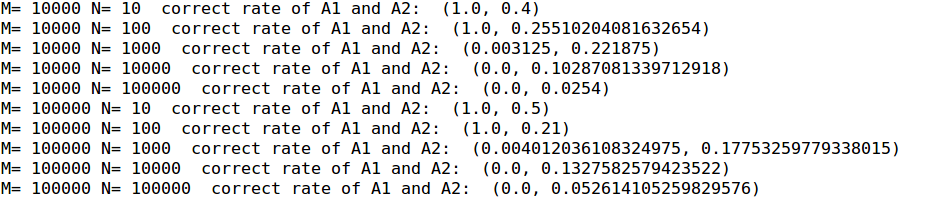
\includegraphics[width=0.6\textwidth]{fixAandB} 
\caption{Uniformly Data Test A and B Fixed}
\end{center}
\end{figure}

In $Figure 1$, there are 10 cases, in which 4 cases shows Algorithm1's correct rate is higher than Algorthm2's and 6 cases shows Algorithm2's correct rate is higher. So in cases that N is not so large, algorithm1's correct rate is higher, as $N$ becomes very larger, we see algorithm2's correct rate is higher.

\subsection{Uniform Distribution, Fix M = 10000 and N = 1000}
In this group of test, we filter out the ones that $A*B>=M$ since it use too much spaces. Then we have $Figure 2$ that shows the test output when we fix $M = 10000$ and $N = 100$.
\begin{figure}[h]
\begin{center}
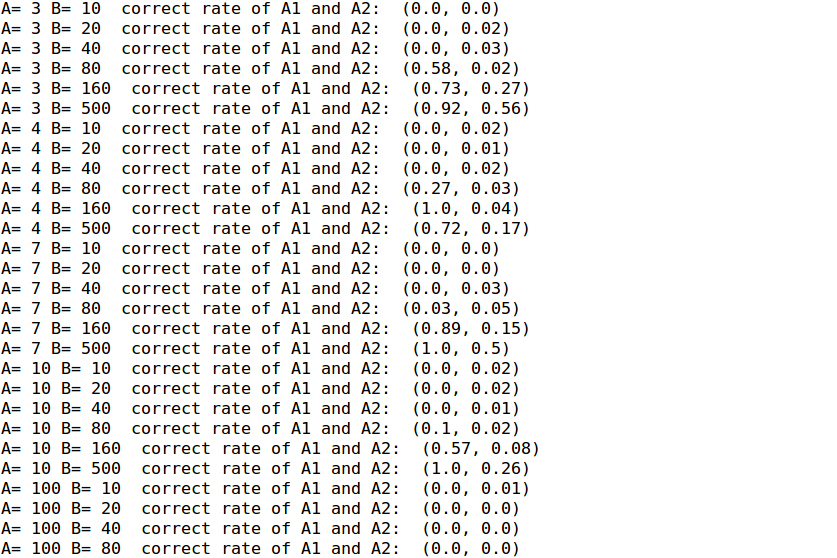
\includegraphics[width=0.6\textwidth]{fixMandN} 
\caption{Uniformly Data Test M and N Fixed}
\end{center}
\end{figure}

From $Figure 2$, we can find that when $B$ is small, such as $B = \{10, 20\}$, the correct rate of algorithm2 is higher, but when $B$ is large, such as $B = \{80, 160, 500\}$, algorithm1 correct rate is higher.

\subsection{Exponential Distribution, Most Frequently Items}
In this group of test, we tested the correct rate of the first 20\% most frequently appeared items in the stream. We first fixed $A=10, B=500$, then fixed $M = 100, N = 1000$. 

\begin{figure}[h]
\begin{center}
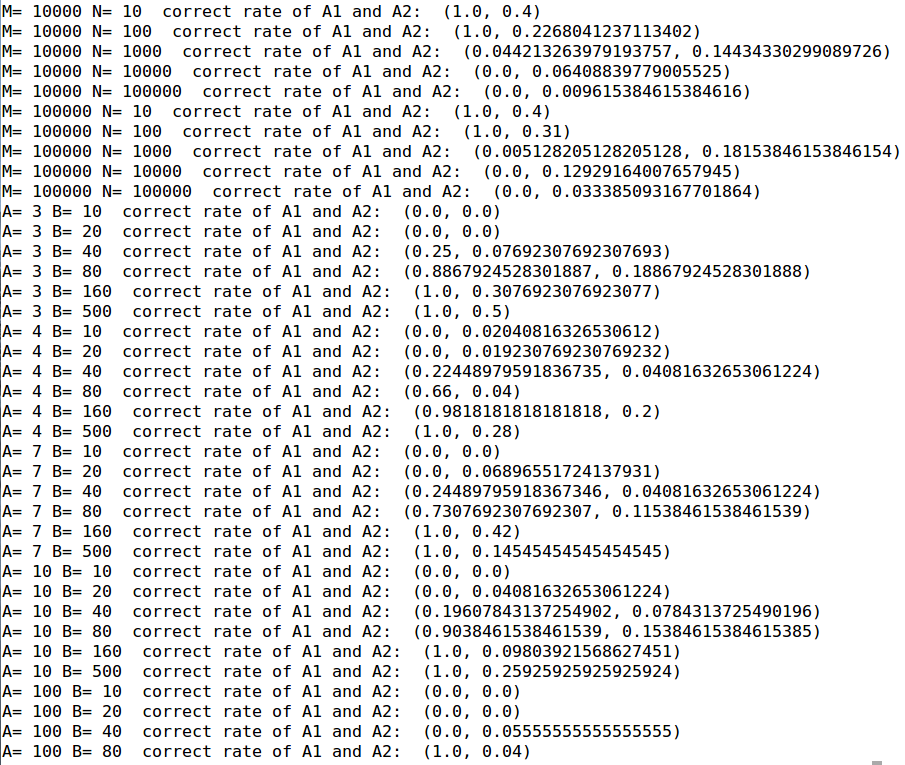
\includegraphics[width=0.6\textwidth]{ExpMost} 
\caption{Exponential Distribution Test on Most Frequently Items}
\end{center}
\end{figure}

Then in $Figure 3$ we find the similar result of comparison of algorithm1 and algorithm2, that when $N$ is large or $B$ is small, algorithm2's correct rate is higher. When $N$ is small and $B$ is large, algorithm1's correct rate is higher.

\subsection{Exponential Distribution, Least Frequently Items}
In this group of test, we tested the correct rate of the last 20\% least frequently appeared items in the stream. The parameters $A, B, M, N$ value setting is the same with 4.3.
\begin{figure}[h]
\begin{center}
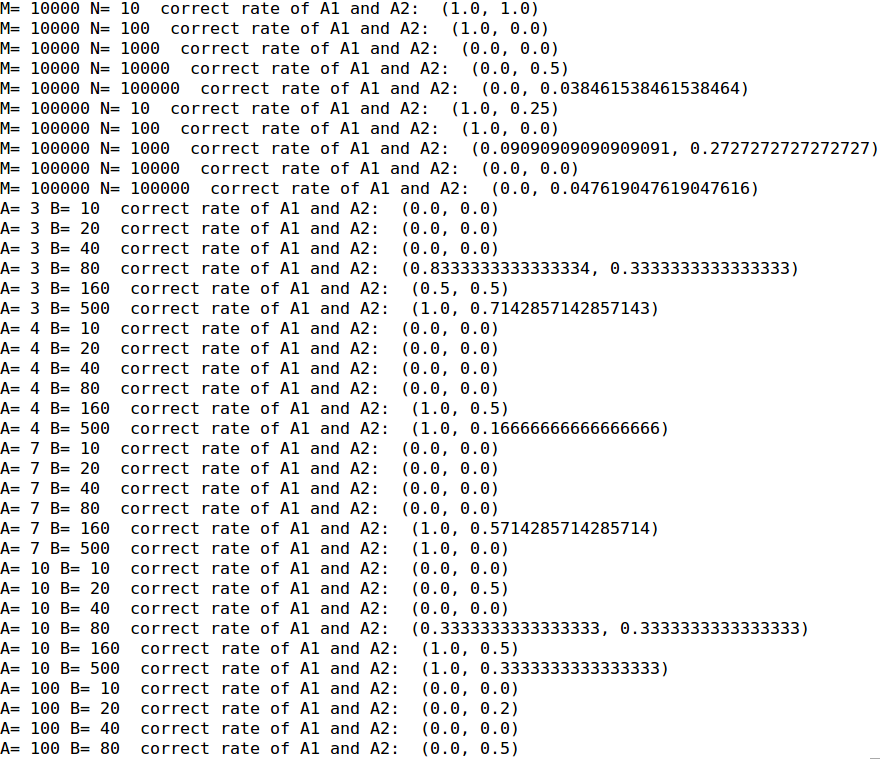
\includegraphics[width=0.6\textwidth]{ExpLeast} 
\caption{Exponential Distribution Test on Least Frequently Items}
\end{center}
\end{figure}
Then in $Figure 4$ we find the same result as we said above other conditions, that when $N$ is large or $B$ is small, algorithm2's correct rate is higher. When $N$ is small and $B$ is large, algorithm1's correct rate is higher. 

\section{Conclusions and Discussion}
From the observation of the experimenting result, I draw conclusions below:
\begin{enumerate}
\item When $N$ is large or when $B$ is small, algorithm2 is more accurate then algorithm1, while algorithm1 perform better when $N$ is small or $B$ is big.
\item The distribution of input stream does not influence which algorithm is better on accuracy.
\item The different elements in the stream does not influence which algorithm is better on accuracy.
\end{enumerate}

I think the reason of conclusion (a) is might because algorithm2 is designed to subtracting some of the noise from nearby counters, so when $N$ is large and $B$ is small, we can easily think of that the noise become bigger, since more items are mapped into smaller buckets.
\newline
\newline
And the reason of conclusion (b) and (c) is might because the hash function we use is random enough(since we choose big enough $Prime$), so no matter how the input data is, we can map them uniformly into our B buckets.  


%----------------------------------------------------------------------------------------
%	BIBLIOGRAPHY
%----------------------------------------------------------------------------------------

\bibliographystyle{apalike}

\bibliography{sample}

%----------------------------------------------------------------------------------------


\end{document}